
% Copyright (c) 2015 - 2020 Mario Mlačak, mmlacak@gmail.com
% Licensed and published as Public Domain work.

% One chapter =========================================================
\chapter*{One}
\addcontentsline{toc}{chapter}{One}

\begin{flushright}
\parbox{0.8\textwidth}{
\emph{God is not external to anyone, but is present with all things, though
they are ignorant that he is so. \\
\hspace*{\fill}{\textperiodcentered \textperiodcentered \textperiodcentered \hspace*{0.2em} Plotinus} } }
\end{flushright}

\noindent
One is chess variant which is played on 26 x 26 board, with white
and darker violet fields, with light purple and fuchsia pieces.
Star colors are the same as for ordinary pieces, i.e. light purple and
fuchsia. In algebraic notation, columns are enumerated from 'a' to 'z',
and rows are enumerated from '1' to '26'. A new piece is introduced,
Starchild.

\clearpage % ..........................................................
% Starchild ***********************************************************

\section*{Starchild}
\addcontentsline{toc}{section}{Starchild}

\noindent
\begin{wrapfigure}{l}{0.4\textwidth}
\centering
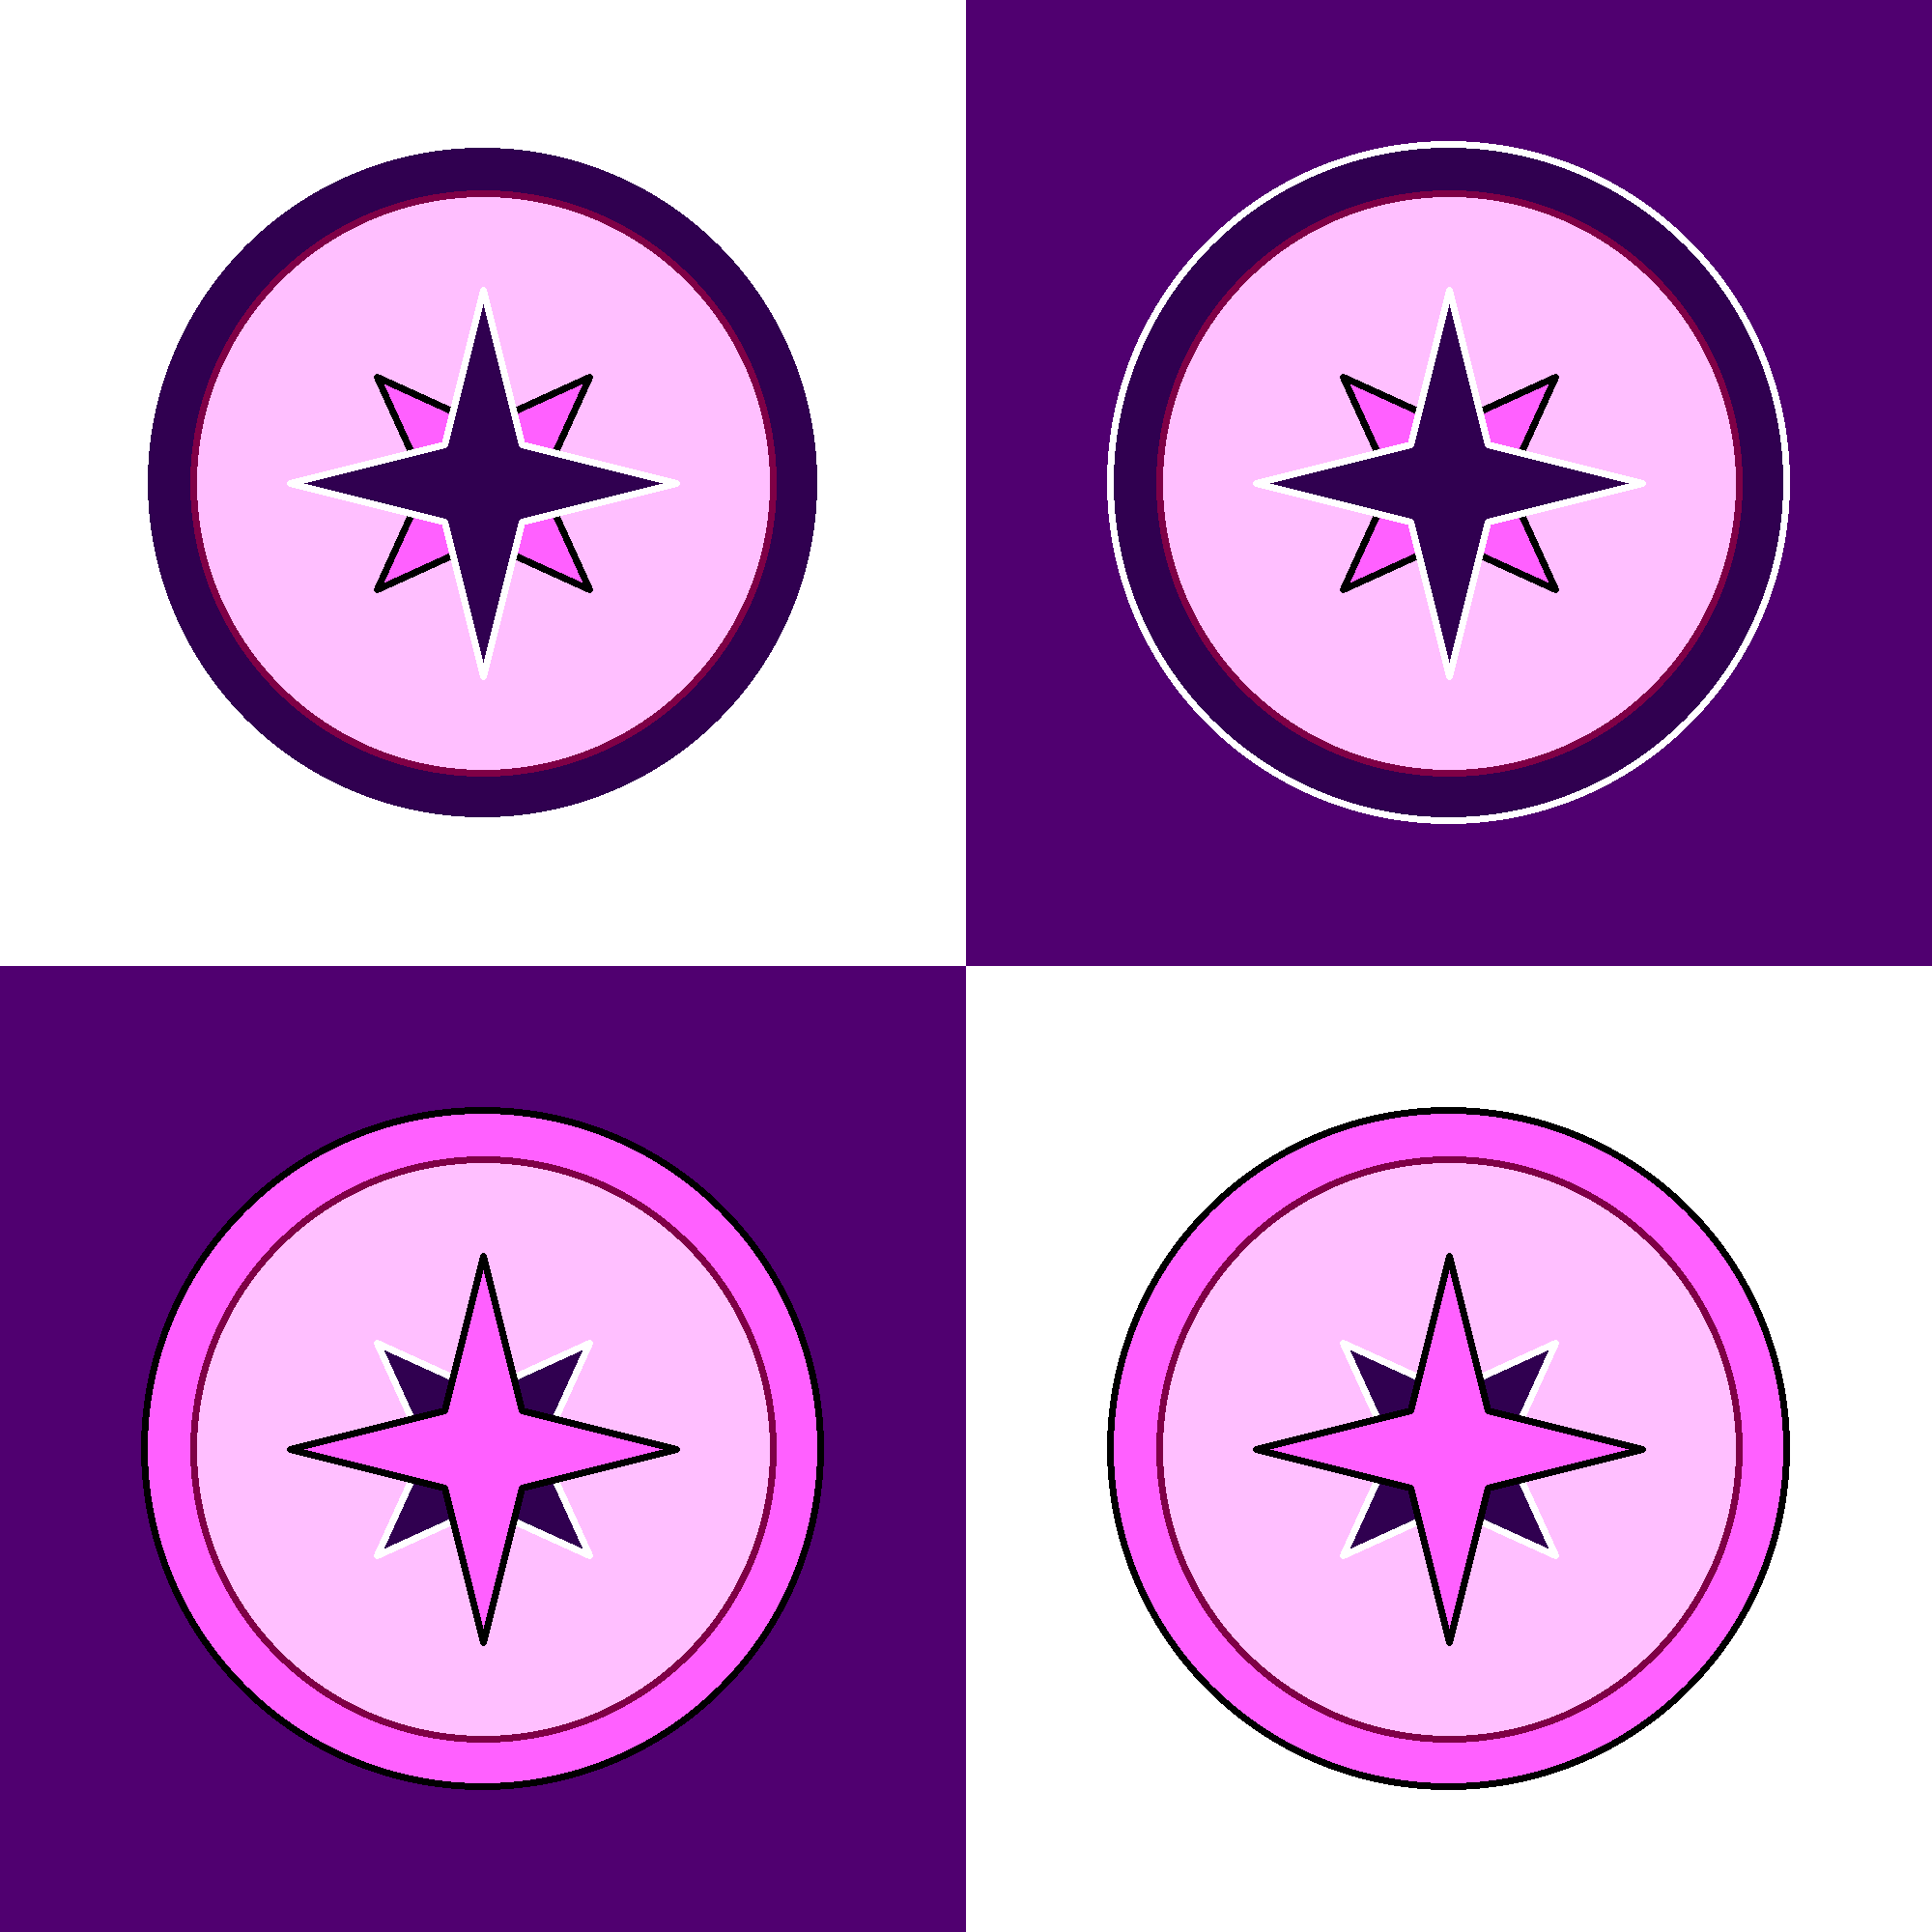
\includegraphics[width=0.4\textwidth, keepaspectratio=true]{pieces/16_starchild.png}
\caption{Starchild}
\label{fig:16_starchild}
\end{wrapfigure}

Starchild cannot be converted, but can be activated.

[?] Starchild does accumulate momentum, but does not spend it while moving. [?]

[*] Syzygy (+?) ... [*]

[*] Starchild moves Stars. [*]

[*] Starchild can tag any piece for (non-destructive?) trance-journey. [*]

[*] Paralel journey (+?) ... [*]

In algebraic notation, symbol for Starchild is 'I'.

[*] TODO :: Star moved --> Wave can pass through ... [*]

% *********************************************************** Starchild
\clearpage % ..........................................................

\section*{Promotion}
\addcontentsline{toc}{section}{Promotion}

Promotion is non enforced, delayed variety, i.e. it's the same as in
\hyperref[sec:Age of Aquarius/Promotion]{previous chess variant}, Age of Aquarius.

Additionaly, promotion in this variant is monogamous.
Only one Queen in the same color can be present on chessboard at any given time.

\clearpage % ..........................................................

\section*{En passant}
\addcontentsline{toc}{section}{En passant}

\noindent
\begin{wrapfigure}{l}{0.4\textwidth}
\centering

\includegraphics[width=0.125\textwidth, keepaspectratio=true]{en_passants/22_one_en_passant.png}
\caption{En passant}
\label{fig:22_one_en_passant}
\end{wrapfigure}
Rush and en passant are identical to those in Classic Chess, only difference
is that Pawn can now move longer on initial turn, up to 11 fields in this
variant.

\clearpage % ..........................................................

\section*{Castling}
\addcontentsline{toc}{section}{Castling}

Castling is the same as in Classical Chess, only difference is that King can move between 2 and 10 fields across.
All other constraints from Classical Chess still applies.

\noindent
\begin{figure}[!h]
% \begin{figure}[!t]
\includegraphics[width=1.0\textwidth, keepaspectratio=true]{castlings/22_o/one_castling.png}
\caption{Castling}
\label{fig:one_castling}
% \centering
\end{figure}

In example above, all valid King's castling moves are numbered.

\noindent
\begin{figure}[!h]
% \begin{figure}[!t]
\includegraphics[width=1.0\textwidth, keepaspectratio=true]{castlings/22_o/one_castling_right_04.png}
\caption{Castling short right}
\label{fig:one_castling_right_04}
% \centering
\end{figure}

In this example King was castling short to the right. Initial King's position is marked with "K".
After castling is finished, right Rook ends up at field immediately left to the King.

\clearpage % ..........................................................

\section*{Initial setup}
\addcontentsline{toc}{section}{Initial setup}

Compared to initial setup of Discovery, Starchild is inserted between Unicorn and Shaman
symmetrically, on both sides of chessboard. This can be seen in the image below:

\noindent
% \begin{figure}[t]
\begin{figure}[h]
\includegraphics[width=1.0\textwidth, keepaspectratio=true]{boards/22_one.png}
\caption{One board}
\label{fig:22_one}
% \centering
\end{figure}

\clearpage % ..........................................................
% ========================================================= One chapter
